\documentclass{article}
\usepackage[utf8]{inputenc}
\usepackage{amsmath}
\usepackage{changepage}
\usepackage{graphicx}
\usepackage{caption}

\title{Growth of Functions}
\begin{document}
\maketitle

\section{Asymptotic Notation}
\begin{adjustwidth}{2.5em}{0pt}
We define a $\Theta$ notation as:
 \begin{equation*}
     \Theta(g(n)) = \{f(n) \hspace{0.1cm}\exists c_1, c_2, n_0,0\leq c_1g(n)\leq(f(n))\leq c_2g(n); \forall n, n\geq  n_0\}
 \end{equation*}
That is, a growth function like a sandwich. Noted that both $f(n)$ and $g(n)$ cannot be negative (\textbf{asymptotically positive})\newline
\textbf{Asymptotically tight bond}: for all $n\geq n_0$, the function $f(n)$ is equal to $g(n)$ to within a constant factor
\begin{center}
        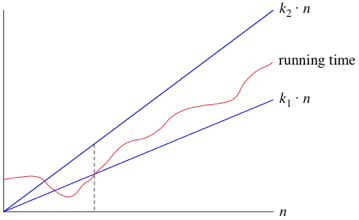
\includegraphics[]{atb.png} 
        \captionof{figure}{Example of an asymptotic tight bond}
\end{center}



\end{adjustwidth}
 
\end{document}
